% Subgrafo real: eventos dos 365 dias anteriores a 2019-01-02, meia-vida de 90 dias.
% Pesos = soma dos eventos com sinal e decaimento (Equação peso-evento).
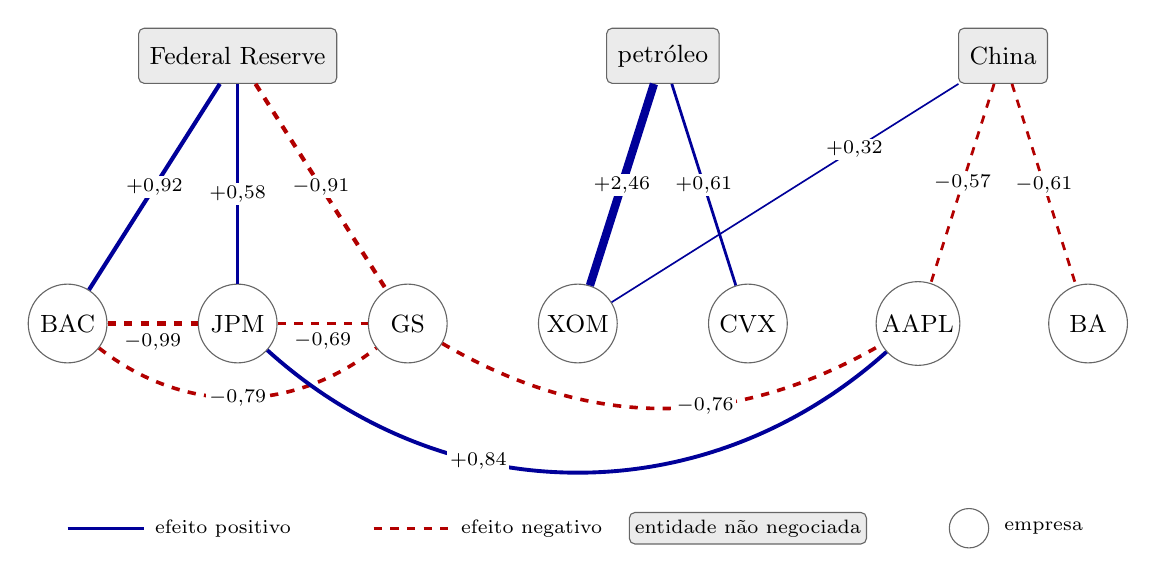
\begin{tikzpicture}[
  x=1.08cm, y=1cm,
  ent/.style={draw=black!60, fill=black!8, rounded corners=2pt, font=\small, inner sep=4pt, minimum height=7mm},
  emp/.style={draw=black!60, fill=white, circle, font=\small, inner sep=1.5pt, minimum size=10mm},
  efpos/.style={draw=blue!60!black},
  efneg/.style={draw=red!70!black, dashed},
  rot/.style={font=\scriptsize, fill=white, inner sep=1pt},
]
% entidades não negociadas
\node[ent] (fed)   at (2,3.4)  {Federal Reserve};
\node[ent] (oil)   at (7,3.4)  {petróleo};
\node[ent] (china) at (11,3.4) {China};
% empresas
\node[emp] (bac)  at (0,0)  {BAC};
\node[emp] (jpm)  at (2,0)  {JPM};
\node[emp] (gs)   at (4,0)  {GS};
\node[emp] (xom)  at (6,0)  {XOM};
\node[emp] (cvx)  at (8,0)  {CVX};
\node[emp] (aapl) at (10,0) {AAPL};
\node[emp] (ba)   at (12,0) {BA};
% exposição a entidades (espessura proporcional ao módulo)
\draw[efpos, line width=1.5pt] (fed) -- node[rot, pos=0.5] {$+0{,}92$} (bac);
\draw[efpos, line width=1.0pt] (fed) -- node[rot, pos=0.55] {$+0{,}58$} (jpm);
\draw[efneg, line width=1.5pt] (fed) -- node[rot, pos=0.5] {$-0{,}91$} (gs);
\draw[efpos, line width=3.0pt] (oil) -- node[rot, pos=0.5] {$+2{,}46$} (xom);
\draw[efpos, line width=1.0pt] (oil) -- node[rot, pos=0.5] {$+0{,}61$} (cvx);
\draw[efpos, line width=0.6pt] (china) -- node[rot, pos=0.3] {$+0{,}32$} (xom);
\draw[efneg, line width=1.0pt] (china) -- node[rot, pos=0.5] {$-0{,}57$} (aapl);
\draw[efneg, line width=1.0pt] (china) -- node[rot, pos=0.5] {$-0{,}61$} (ba);
% arestas diretas entre empresas
\draw[efneg, line width=1.5pt] (bac) -- node[rot, below=2pt] {$-0{,}99$} (jpm);
\draw[efneg, line width=1.2pt] (jpm) -- node[rot, below=2pt] {$-0{,}69$} (gs);
\draw[efneg, line width=1.3pt] (bac) to[bend right=38] node[rot] {$-0{,}79$} (gs);
\draw[efneg, line width=1.3pt] (gs) to[bend right=30] node[rot, pos=0.6] {$-0{,}76$} (aapl);
\draw[efpos, line width=1.4pt] (jpm) to[bend right=42] node[rot, pos=0.35] {$+0{,}84$} (aapl);
% legenda
\draw[efpos, line width=1.2pt] (0,-2.6) -- (0.9,-2.6) node[right, font=\scriptsize, black] {efeito positivo};
\draw[efneg, line width=1.2pt] (3.6,-2.6) -- (4.5,-2.6) node[right, font=\scriptsize, black] {efeito negativo};
\node[ent, minimum height=4mm, inner sep=2pt, font=\scriptsize] at (8.0,-2.6) {entidade não negociada};
\node[emp, minimum size=5mm, font=\scriptsize] at (10.6,-2.6) {};
\node[right, font=\scriptsize] at (10.9,-2.6) {empresa};
\end{tikzpicture}
